\section{Voltage Divider}

One of them most important circuits in electronics is the voltage divider as depicted in \cref{fig:simple-voltage-divider}. In this circuit two resistors $R_1$ and $R_2$ are between connected in series between a voltage source $V_{cc}$ and Ground. Because this is a closed circuit there is a current flowing through the resistors and each resistor is responsible for an individual voltage drop. Can we calculate the voltage $U_o$ between these two resistors?

It is simple to see that the current flowing in this circuit is the same for both resistors. When two resistors are connected in series their resistances sum up and this total resistance can be used to calculate the current with Ohms law:
\begin{equation*}
	I = \frac{U}{R} = \frac{V_{cc}}{R_1 + R_2}\,.
\end{equation*}
We also know that the voltage drop $U_1$ across $R_1$ and the voltage drop $U_2$ across $R_2$ sum up to the supply voltage: $U_1 + U_2 = V_{cc}\,$. The voltage drop across $R_2$ can be calculated using Ohms law again because we know the current and the resistance:
\begin{equation*}
	U_2 = R \cdot I = V_{cc} \cdot \frac{R_2}{R_1 + R_2}\,.
\end{equation*}
A similar behavior can be seen for $R_1$:
\begin{equation*}
	U_1 = R \cdot I = V_{cc} \cdot \frac{R_1}{R_1 + R_2}\,.
\end{equation*}

This shows us that we can calculate the voltage $U_o = U_2 = V_{cc} - U_1$ between the resistors. It is independent from the total current and only depending on the ratio of the two resistors. It would not make a difference if we use $R_1 = \SI{10}{K\Omega}, R_2 = \SI{2,2}{K\Omega}$ or $R_1 = \SI{10}{\Omega}, R_2 = \SI{2,2}{\Omega}$, the result would be the same.


\begin{figure}[htb]
	\centering
	\begin{tikzpicture}
		\draw (0,0) node[ground] {}
			to[resistor, l=$R_2$, -*] ++ (0,2) coordinate (A)
			to[short, -o] ++ (1,0)
			node[auto, anchor=west] {$U_o$}
			(A) to[resistor, l=$R_1$] ++ (0,2)
			node[vcc] {$V_{cc}$}
		;
	\end{tikzpicture}
	\caption{A voltage divider made with two resistors}
	\label{fig:simple-voltage-divider}
\end{figure}


The characteristic equation to describe a voltage divider can be seen in \cref{equ:resistive-voltage-divider}:
\begin{equation}
	\frac{U_1}{U_2} = \frac{R_1}{R_2}\,.
	\label{equ:resistive-voltage-divider}
\end{equation}

We can use this circuit to reduce a voltage but its usability as a voltage source is limited. This can be shown in \cref{fig:loaded-voltage-divider} by adding a load, in this case a resistor $R_L$. Now the total resistance of the parallel resistors $R_2$ and $R_L$ calculates to
\begin{equation*}
	R_x = R_2 \parallel R_L = \frac{1}{\frac{1}{R_2} + \frac{1}{R_L}}
\end{equation*}
and the result of this is smaller than $R_2$ and $R_L$. The load changes the voltage divider and this changes the output voltage $U_o$.


\begin{figure}[htb]
	\centering
	\begin{tikzpicture}
		\draw (0,0) node[ground] {}
			to[resistor, l=$R_2$, -*] ++ (0,2) coordinate (A)
			to[short, -o] ++ (1,0) coordinate (B)
			node[auto, anchor=west] {$U_o$}
			(A) to[resistor, l=$R_1$] ++ (0,2)
			node[vcc] {$V_{cc}$}
			(B) to[resistor, l=$R_L$] ++ (0,-2)
			to[short, -*] ++ (-1,0)
		;
	\end{tikzpicture}
	\caption{A voltage divider with load resistance}
	\label{fig:loaded-voltage-divider}
\end{figure}

A voltage divider can only be used as a voltage source if there is no load attached to it. This means we cannot use it to drive an electric device but we will later see that there is a possibility to avoid this issue.

Right now we only have discussed what happens when we have a fixed voltage $V_{cc}$ driving this circuit. With an AC supply $U = U_0 \cdot \sin(\omega \cdot t)$ the voltage divider still works the same because only $V_{cc}$ is time dependant, the resistors are constant and independent from the voltage or the frequency of $V_{cc}$ and therefore it should work the same with AC and DC current.

\begin{figure}[htb]
		\centering
		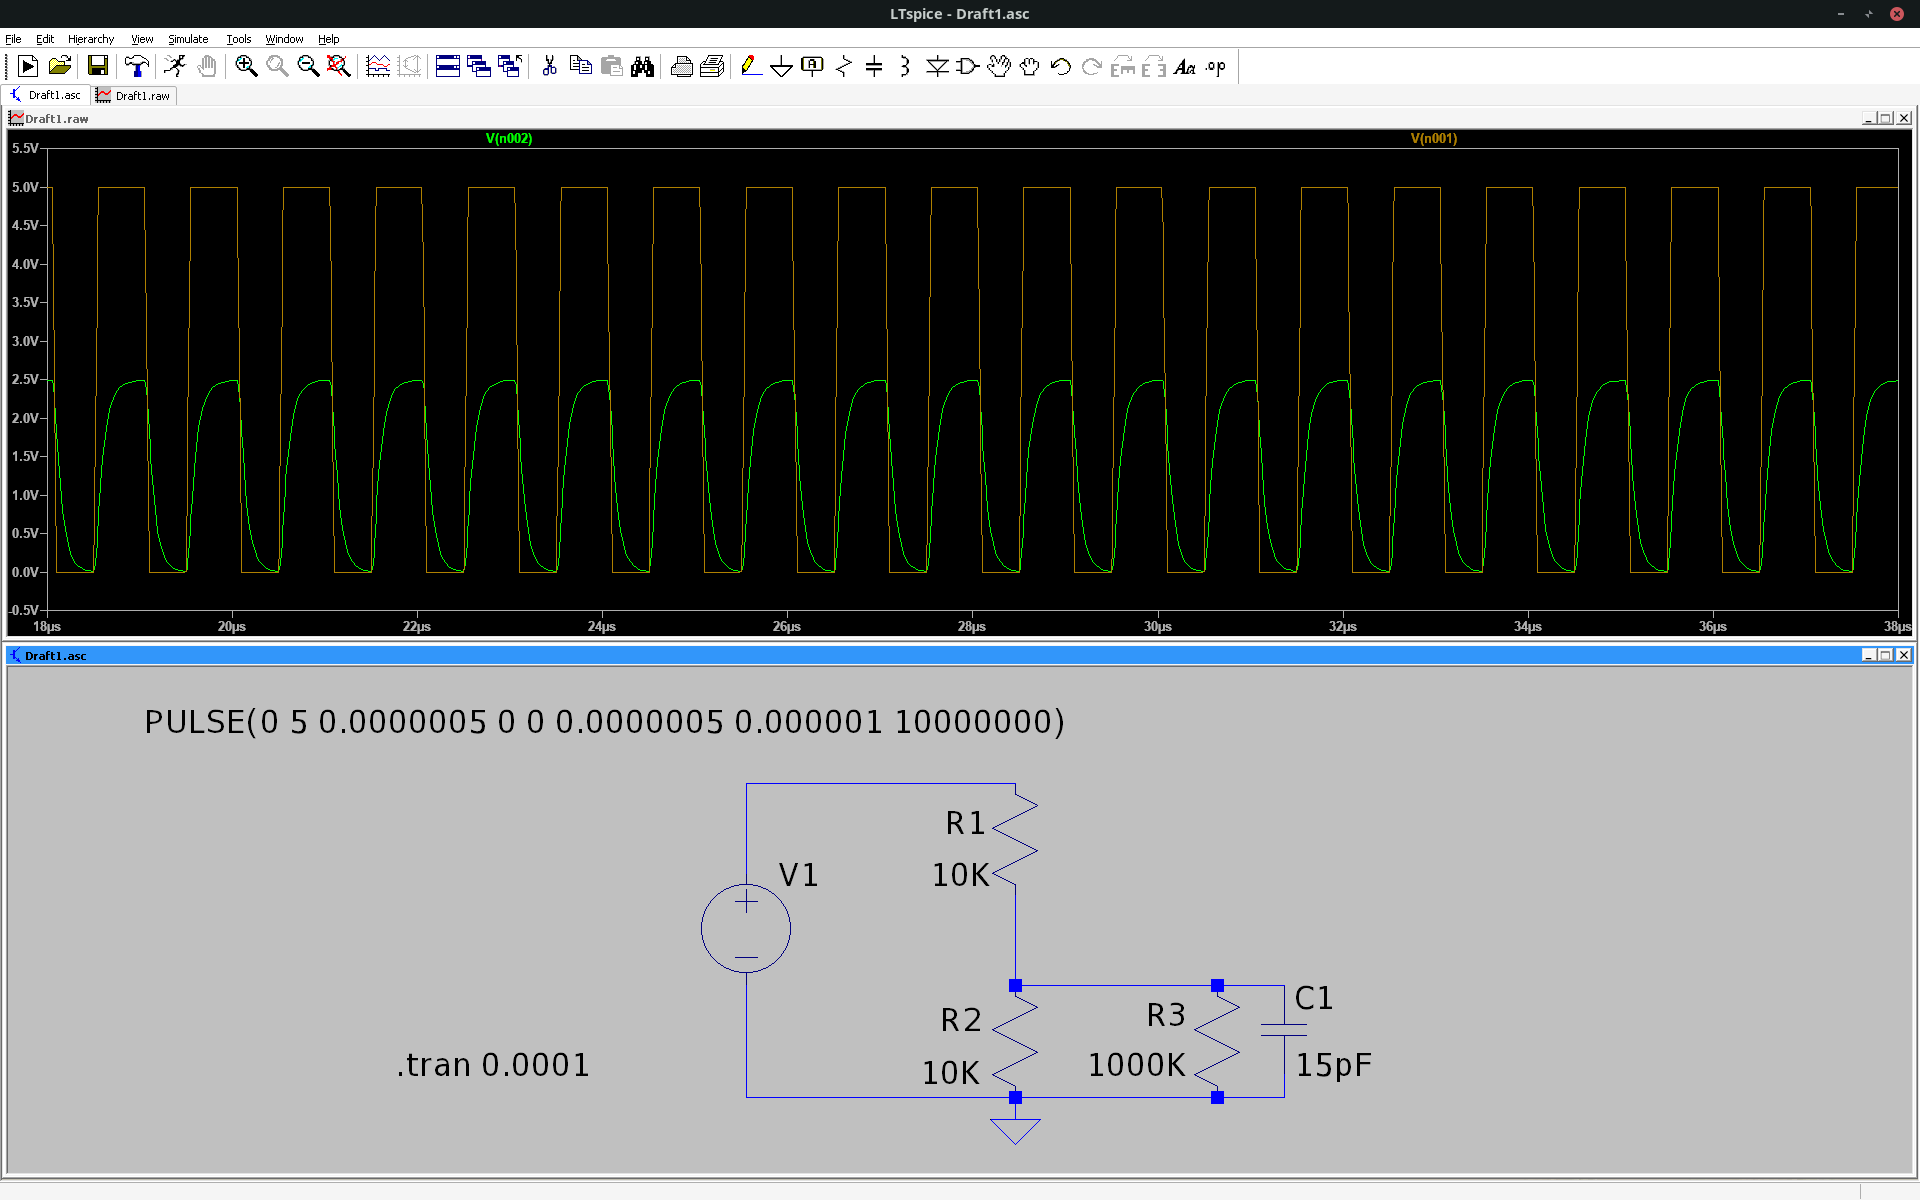
\includegraphics[width=0.8\textwidth]{voltage-divider-distortion-simulation.png}
		\caption{A square wave signal which is being disturbed by the input capacitance of an ADC}
		\label{fig:voltage-divider-distortion}
\end{figure}

Hold on! The last paragraph was partially a lie. In theory a resistor should only have a resistance but in reality every component has some resistance, capacitance and inductance. In many cases we can ignore the unwanted side-effects but when the circuit has to interact with high frequency signals these have to be taken into account. If we want to measure the voltage $U_o$ then our measurement device (which would be an ADC) has a large input resistance and a small input capacity. The large input resistance is good because ifs effect on the voltage divider can be neglected\footnote{You wanna know why? Calculate the reduction of an input voltage for a 1:1 voltage divider made out of $\SI{1}{K\Omega}$ resistors with and without an $R_L = \SI{10}{M\Omega}$ load.} but the small input capacitance would introduce a new side effect on this circuit. \cref{fig:voltage-divider-distortion} is a simulation of a square signal which will be distorted by the small input capacitance ($C_1 = \SI{15}{pF}$) of a measurement device (The large input resistance $R_3 = \SI{1}{M\Omega}$ was also taken into account in this simulation). Before we discuss how to deal with this side effect we will take a look on a voltage divider which is build especially for AC currents.


\subsection{The capacitive voltage divider}

For a DC voltage a capacitor is an impervious barrier but for an AC voltage the capacitor behaves like an electrical conductor which induces a phase shift of $\SI{90}{\degree}$. If we arrange two capacitors as seen in \cref{fig:capacitive-voltage-divider} and have an alternating voltage $\sim V_{cc}$ we can observe an similar behavior as with the resistor based voltage divider in \cref{fig:simple-voltage-divider}.


\begin{figure}[htb]
	\centering
	\begin{tikzpicture}
		\draw (0,0) node[ground] {}
			to[C, l=$C_2$, -*] ++ (0,2) coordinate (A)
			to[short, -o] ++ (1,0)
			node[auto, anchor=west] {$U_o$}
			(A) to[C, l=$C_1$] ++ (0,2)
			node[vcc] {$\sim V_{cc}$}
		;
	\end{tikzpicture}
	\caption{A capacitive voltage divider}
	\label{fig:capacitive-voltage-divider}
\end{figure}


In this circuit the overall charge $Q$ through the capacitors is preserved:
\begin{equation*}
	Q = C \cdot U = C_1 \cdot U_1 = C_2 \cdot U_2\,
\end{equation*}
where $U_1$ and $U_2$ are the voltage drops across the capacitors $U_1$ and $U_2$. With the overall capacity of two capacitors in series:
\begin{equation*}
	C_x = \frac{1}{\frac{1}{C_1} + \frac{1}{C_2}} = \frac{C_1 \cdot C_2}{C_1 + C_2}
\end{equation*}
and the use of $Q = C_x \cdot V_{cc} = C_2 \cdot U_2$ the voltage $U_2$ drop across $C_2$ can be calculated:
\begin{equation*}
	U_2 = U_0 \frac{Q}{C} =  \frac{V_{cc}}{C_2} \cdot C_x = \frac{V_{cc}}{C_2} \cdot \frac{C_1 \cdot C_2}{C_1 + C_2} = V_{cc} \cdot \frac{C_1}{C_1 + C_2}
\end{equation*}
From symmetric reasons the equation for $U_1$ looks similar:
\begin{equation*}
	U_1 =  V_{cc} \cdot \frac{C_2}{C_1 + C_2}
\end{equation*}

From this the characteristic equation of the capacitive voltage divider is \cref{equ:capacitive-voltage-divider}

\begin{equation}
	\frac{U_1}{U_2} = \frac{C_2}{C_1}\,.
	\label{equ:capacitive-voltage-divider}
\end{equation}

With this knowledge we can build a voltage divider for AC signals but it cannot be used for DC voltages. Like a resistive voltage divider a capacitive one also only works when there is no load attached. A load can also be seen as an additional capacitor, similar to \cref{fig:loaded-voltage-divider}, which changes the capacitance ration and affects the voltage drop.


\subsection{Frequency compensated attenuator}

A resistive attenuator can only be used properly with DC voltages or AC voltages at low frequencies and a capacitive attenuator can be used with alternating voltages at high frequencies but is unusable for DC voltages. The solution to achieve both within a single circuit is called a "Frequency compensated attenuator" (\textit{attenuator} is just another name for a voltage divider).


\begin{figure}[htb]
	\centering
	\begin{tikzpicture}
		\draw (0,0) node[ground] {}
			to[short, *-] ++ (-2,0)
			to[resistor, l=$R_2$] ++ (0,2) coordinate (A)
			to[resistor, l=$R_1$, *-] ++ (0,2)
			-- ++ (2,0)
			node[vcc] {$V_{cc}$}
			to[short, *-] ++ (0,0)
			to[C, l=$C_1$, -*] ++ (0,-2) coordinate (B)
			to[C, l=$C_2$, -*] ++ (0,-2)
			-- ++ (-1,0)
			(B) ++ (2,0) coordinate (C)
			to[vC, l=$C_T$, *-] ++ (0,-2)
			to[short, -*] ++ (-2,0)
			(A) to[short] (B)
			to[short] (C)
			to[short, -o] ++ (1,0)
			node[auto, anchor=west] {$U_o$}
		;
	\end{tikzpicture}
	\caption{A frequency compensated attenuator with an adjustable capacitor for fine tuning}
	\label{fig:frequency-compensated-attenuator}
\end{figure}

The attenuator in \cref{fig:frequency-compensated-attenuator} is just a combination of a resistive voltage divider for DC signals and a capacitive voltage divider for AC signals in parallel. By using resistors which are way smaller than the load resistance of a measurement device the load would not affect this attenuator. The same thing happens when the capacitors are chosen large enough: a small load capacity would not effect the attenuator. There is also a trimmer capacitor which will be discussed later.

Let's take a look at the behaviour of this voltage divider first. We know the descriptive formulas of the previously discussed voltage dividers:
\begin{equation*}
	\frac{U_1}{U_2} = \frac{R_1}{R_2} = \frac{C_2}{C_1}
\end{equation*}
This means that a frequency compensated attenuator needs to fulfill the following requirements:
\begin{equation}
	R_1 \cdot C_1 = R_2 \cdot C_2\,.
	\label{equ:frequency-compensated-attenuator}
\end{equation}
This equation is essential for choosing the right components. One missing detail lies in the trimmer capacitor. Its only task is to compensate uncertainties of the components or other side effects which have not been taken into account. This trimmer capacitor can be set to its proper value in a calibration process until \cref{equ:frequency-compensated-attenuator} is satisfied. To do so the attenuator needs to be driven by a square signal. During a recording of $U_o$ the trimmer capacitor needs to be adjusted until the results show a pure square signal with no distortions.


\subsection{Adding voltages}

In \cref{fig:simple-voltage-divider} the voltage divider was constructed in a way where the second resistor was connected to ground. This makes it easy to calculate $U_o$ which is the voltage drop across $R_2$ added to the electrical potential at the other side of the resistor: $U_o = U_{Gnd} + U_2\,$. Since the grounding is just a fixed value for a potential this could also be set to an arbitrary value above or below Ground and the voltage divider would still work on the potential difference across the two resistors. We are going to abuse this effect to shape the output signal of the attenuator.

An ADC can only convert voltages from $\SI{0}{V}$ up to a reference voltage $U_{ref}$. To accept higher voltages than $U_{ref}$ an attenuator can be used to reduce the voltage by a factor which is specified by the resistor ratio. For voltages below the Ground of the ADC the only option is to shift the voltage up by adding a DC offset. Replacing the Ground potential at the attenuator with a Voltage source makes this voltage addition possible.

\begin{figure}[htb]
	\centering
	\begin{tikzpicture}
		\draw (0,0) node[vcc] {$V_+$}
			-- ++ (-1,0)
			to[resistor, l=$R_2$, -*] ++ (0,2) coordinate (A)
			to[short, -o] ++ (1,0)
			node[auto, anchor=west] {$U_o$}
			(A) to[resistor, l=$R_1$] ++ (0,2)
			-- ++ (1,0)
			node[vcc] {$V_{in}$}
		;
	\end{tikzpicture}
	\caption{Using an attenuator to add a DC offset to an input voltage}
	\label{fig:attenuator-voltage-adder}
\end{figure}

\cref{fig:attenuator-voltage-adder} is a schematic of this idea. This also works with a capacitive attenuator but for simplicity the calculations will only be done for a resistive attenuator. The overall voltage across both resistors has now changed from $V_{cc} - GND = V{cc} - \SI{0}{V} = V_{cc}$ to the new voltage $U = U_{in} - U_+$. The voltage drop across both resistors stays the same as before, just the input voltage needs to be replaced in this formula:
\begin{equation*}
	U_2 = U \cdot \frac{R_2}{R_1 + R_2} = (U_{in} - U_+) \cdot \frac{R_2}{R_1 + R_2}
\end{equation*}
but $U_2$ is only the voltage drop across $R_2$. We know that the electrical potential has a value of $U_+$ after the current coming from the input signal has passed $R_2$ and we know that it lost a voltage of $U_2$ on its way through $R_2$:
\begin{align*}
	U_o &= U_+ + U_2 = U_+ + (U_{in} - U_+) \cdot \frac{R_2}{R_1 + R_2} \\
		&= U_{in} \cdot \frac{R_2}{R_1 + R_2} + U_+ \left(1 - \frac{R_2}{R_1 + R_2}\right) \\
		&= U_{in} \cdot \frac{R_2}{R_1 + R_2} + U_+ \cdot \frac{R_1}{R_1 + R_2}\,.
\end{align*}
We have shown that this change to the attenuator adds a DC offset of $U_+ \cdot \frac{R_1}{R_1 + R_2}$ to the output voltage $U_0$. This can be used to transform an AC input signal from $\pm U_{in}$ to a range between $\SI{0}{V}$ and the reference voltage $U_{ref}$ of an ADC which makes the signal $\pm U_{in}$ measurable with an ADC. If we want to realise this idea we need to calculate the right values for the resistors and $U_+$.

For our usage we assume that we want to combine an attenuator with a reference Voltage $U_+$ to transform input signals from $\pm{}U_{in}$ which are way above and below the input range of an ADC into a measurable range from $\SI{0}{V}$ to $U_{Aref}$. We want to calculate the right resistor values and reference voltage for a given $\pm{}U_{in}$ and $U_{Aref}$. Therefore we have to take a look at the two cases $+U_{in}$ and $-U_{in}$ where the output voltage of the attenuator should match $U_{Aref}$ and $\SI{0}{V}$.

In the first case we want the maximum value $+U_{in}$ to be mapped to $U_{Aref}$:
\begin{align}
	U_{Aref} &= \lvert U_{in} \rvert \cdot \frac{R_2}{R_1 + R_2} + U_+ \cdot \frac{R_1}{R_1 + R_2} \\
	U_+ \cdot \frac{R_1}{R_1 + R_2} &= U_{Aref} - \lvert U_{in} \rvert \cdot \frac{R_2}{R_1 + R_2}
\end{align}
and in the second case the minimum value $-U_{in}$ to be equal to Gnd:
\begin{align}
	\text{Gnd} &= - \lvert U_{in} \rvert \cdot \frac{R_2}{R_1 + R_2} + U_+ \cdot \frac{R_1}{R_1 + R_2} \\
	U_+ \cdot \frac{R_1}{R_1 + R_2} &= \text{Gnd} + \lvert U_{in} \rvert \cdot \frac{R_2}{R_1 + R_2} = \lvert U_{in} \rvert \cdot \frac{R_2}{R_1 + R_2}\,.
	\label{equ:attenuator_with_offset_derivation}
\end{align}
For simplicity we set Ground to $\SI{0}{V}$ and we can combine the equations:
\begin{align}
	\lvert U_{in} \rvert \cdot \frac{R_2}{R_1 + R_2} &= U_{Aref} - \lvert U_{in} \rvert \cdot \frac{R_2}{R_1 + R_2} \\
	2 \cdot \lvert U_{in} \rvert \cdot \frac{R_2}{R_1 + R_2} &= U_{Aref} \\
	2 \cdot \lvert U_{in} \rvert &= U_{Aref} \cdot \frac{R_1 + R_2}{R_2} = U_{Aref} \cdot \left( \frac{R_1}{R_2} + 1 \right) \\
	2 \cdot \frac{\lvert U_{in} \rvert}{U_{Aref}} &= \frac{R_1}{R_2} + 1 \\
	\frac{R_1}{R_2} &= \frac{2 \cdot \lvert U_{in} \rvert}{U_{Aref}} - 1\,.
\end{align}
This equation shows us that, independent from the voltage shift we can choose a value for one resistor and get the implicit value for the other resistor. The value for the voltage shift can be calculated after the resistor values have been selected. This will be shown with a modification of \cref{equ:attenuator_with_offset_derivation}:
\begin{align}
	U_+ \cdot \frac{R_1}{R_1 + R_2} &= \lvert U_{in} \rvert \cdot \frac{R_2}{R_1 + R_2} \\
	U_+ &= \lvert U_{in} \rvert \cdot \frac{R_2}{R_1 + R_2} \cdot \frac{R_1}{R_1 + R_2} \\
			&= \lvert U_{in} \rvert \cdot \frac{R_2}{R_1}\,.
\end{align}
With these equations we can easily choose the right values for the resistors and the offset voltage when we have decided on the input voltages we want to measure with an ADC. The offset voltage can be provided with an Operational Amplifier.


